% Presentation structure
%
% Part I: Preliminaries
%   The @Web platform
%   @Web ontology
%   Annotated tables
%   Guidelines
%   Examples constraints
%
% Part II: RDF data validation: survey of the state of the art
%   Shape Expressions
%   SHACL
%   Plain SPARQL
%
% Part III: Implementation
%   Examples of real constraints
%   Live demo
%
% Part IV: Conclusions
%   Conclusions
%   Future work
%   Thanks

\documentclass{beamer}
\usepackage[utf8]{inputenc}
\usepackage{graphicx}
\usepackage{xspace}
\usepackage{fancyvrb} % Needed for \verbatim environment
\usepackage{hyperref} % Needed for \href

% Convenience macros
\newcommand{\atweb}{\textbf{@Web}\xspace}
\newcommand{\partslide}[2]{
  \begin{center}
    \LARGE{#1} \\
    \vspace{0.5cm}
    \huge{#2}
  \end{center}
}
\newcommand{\fnhref}[2]{\href{#2}{#1}\footnote{\url{#2}}}
\newcommand{\ifnhref}[2]{\textit{\fnhref{#1}{#2}}}

% Remove navigation controls
\usenavigationsymbolstemplate{}

% Slide numbering
\setbeamertemplate{footline}[frame number]

\title{Using SPARQL queries to express integrity constraints in RDF graphs}
\subtitle{
  \vspace{0.5cm}
  Final internship report
}
\author{
  Leandro Lovisolo
}
\date{February 25, 2016}
\institute{
  INRA SupAgro and INRIA GraphiK \\
  Montpellier, France
}

\begin{document}

\begin{frame}
  \titlepage
\end{frame}

%%%%%%%%%%%%%%%%%%%%%%%%%%%%%%%%%%%%%%%%%%%%%%%%%%%%%%%%%%%%%%%%%%%%%%%%%%%%%%%%
% Part I: Preliminaries                                                        %
%%%%%%%%%%%%%%%%%%%%%%%%%%%%%%%%%%%%%%%%%%%%%%%%%%%%%%%%%%%%%%%%%%%%%%%%%%%%%%%%

\begin{frame}
  \partslide{Part I}{Preliminaries}
\end{frame}

\begin{frame}
  \frametitle{Problem statement}

  \begin{itemize}
    \item We have an RDF graph where we store experimental data extracted from
      tables in scientific publications.

    \item The data extraction process is done semi-manually, thus it's very
      error-prone.

    \item Therefore, \textbf{we want to verify the integrity of the annotated
      data automatically.}
  \end{itemize}
\end{frame}

\begin{frame}
  \frametitle{The \atweb platform}
  \framesubtitle{Introduction}

  \begin{itemize}
    \item A software platform used to annotate tables from scientific
      publications in heterogeneous formats (PDF files, Excel spreadsheets,
      etc.)

    \item Data is stored in an RDF graph following a predefined OWL ontology.

    \item Goal of my internship: add integrity constraint checking capabilities
      to the \fnhref{\atweb
      platform}{http://www6.inra.fr/cati-icat-atweb/Web-platform}.
  \end{itemize}
\end{frame}

\begin{frame}
  \frametitle{The \atweb platform}
  \framesubtitle{Screenshot}

  \begin{center}
    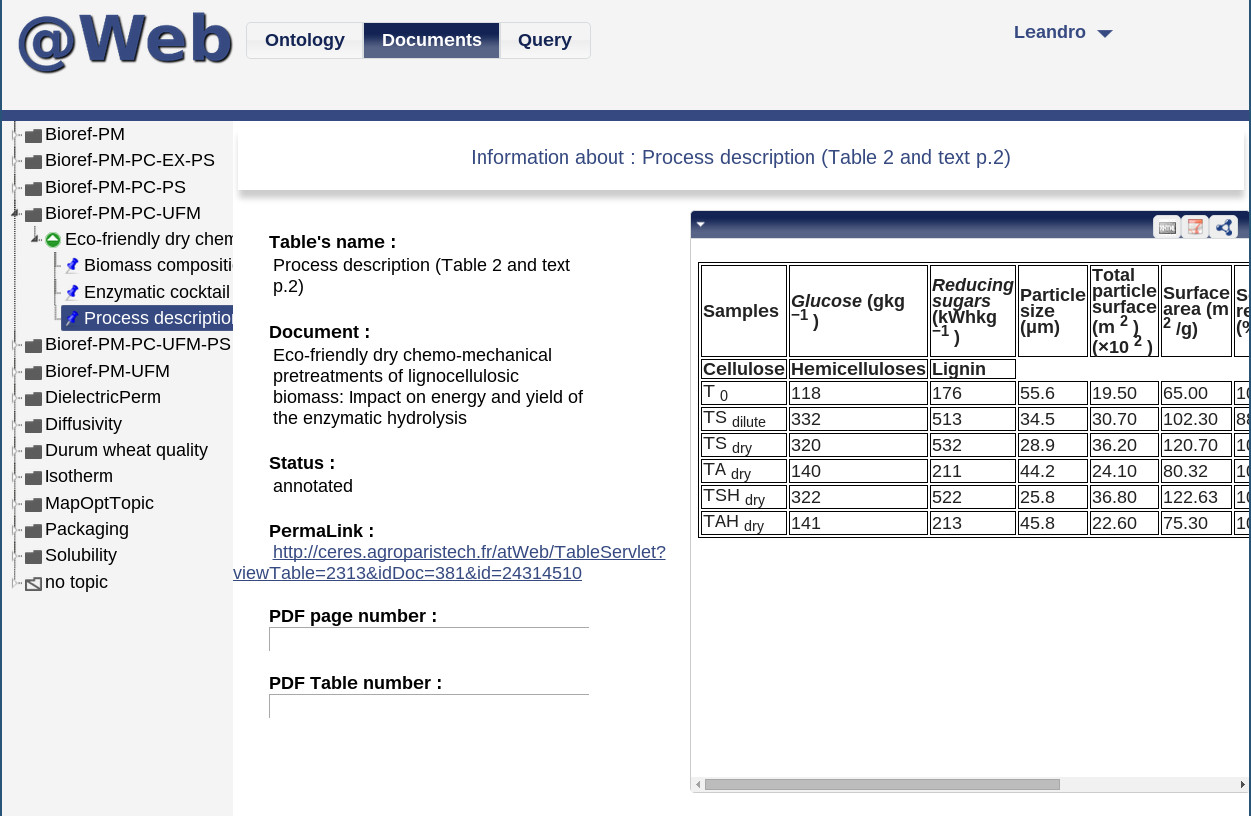
\includegraphics[width=10cm]{atweb-screenshot-document.jpg}
  \end{center}
\end{frame}

\begin{frame}
  \frametitle{The \atweb platform}
  \framesubtitle{$n$-ary relation pattern}

  \begin{itemize}
    \item We're trying to represent experiments composed of many inputs and a
      single output.

    \item An OWL ontology is created where OWL classes are defined for each
      kind of experiment we're interested in representing.

    \item Instances of each experiment class are connected to their respective
      input arguments and output argument via OWL object and data properties.

    \item We're thus defining a pattern for $n$-ary relations.
  \end{itemize}
\end{frame}

\begin{frame}
  \frametitle{The \atweb platform}
  \framesubtitle{Example $n$-ary relation}

  \begin{center}
    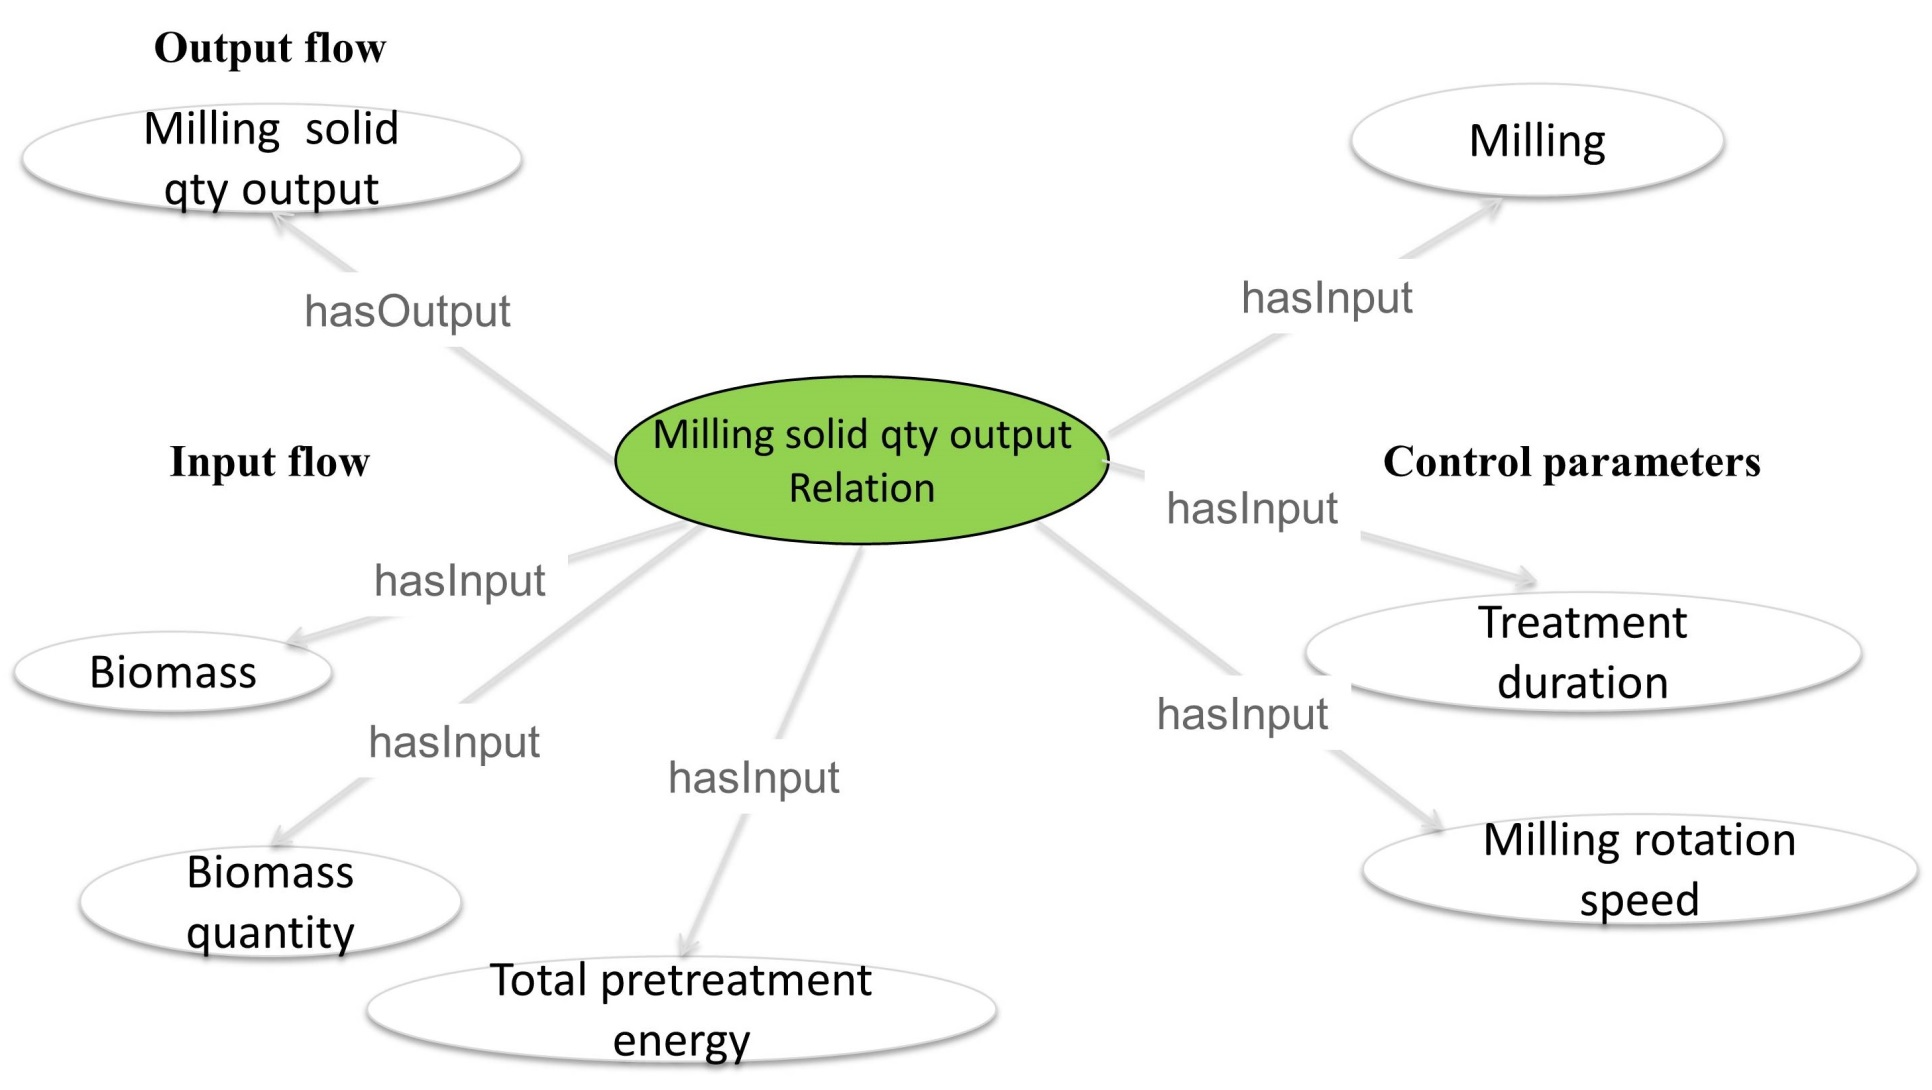
\includegraphics[width=10cm]{relation.jpg}
  \end{center}
\end{frame}

\begin{frame}
  \frametitle{\atweb ontology}

  \begin{center}
    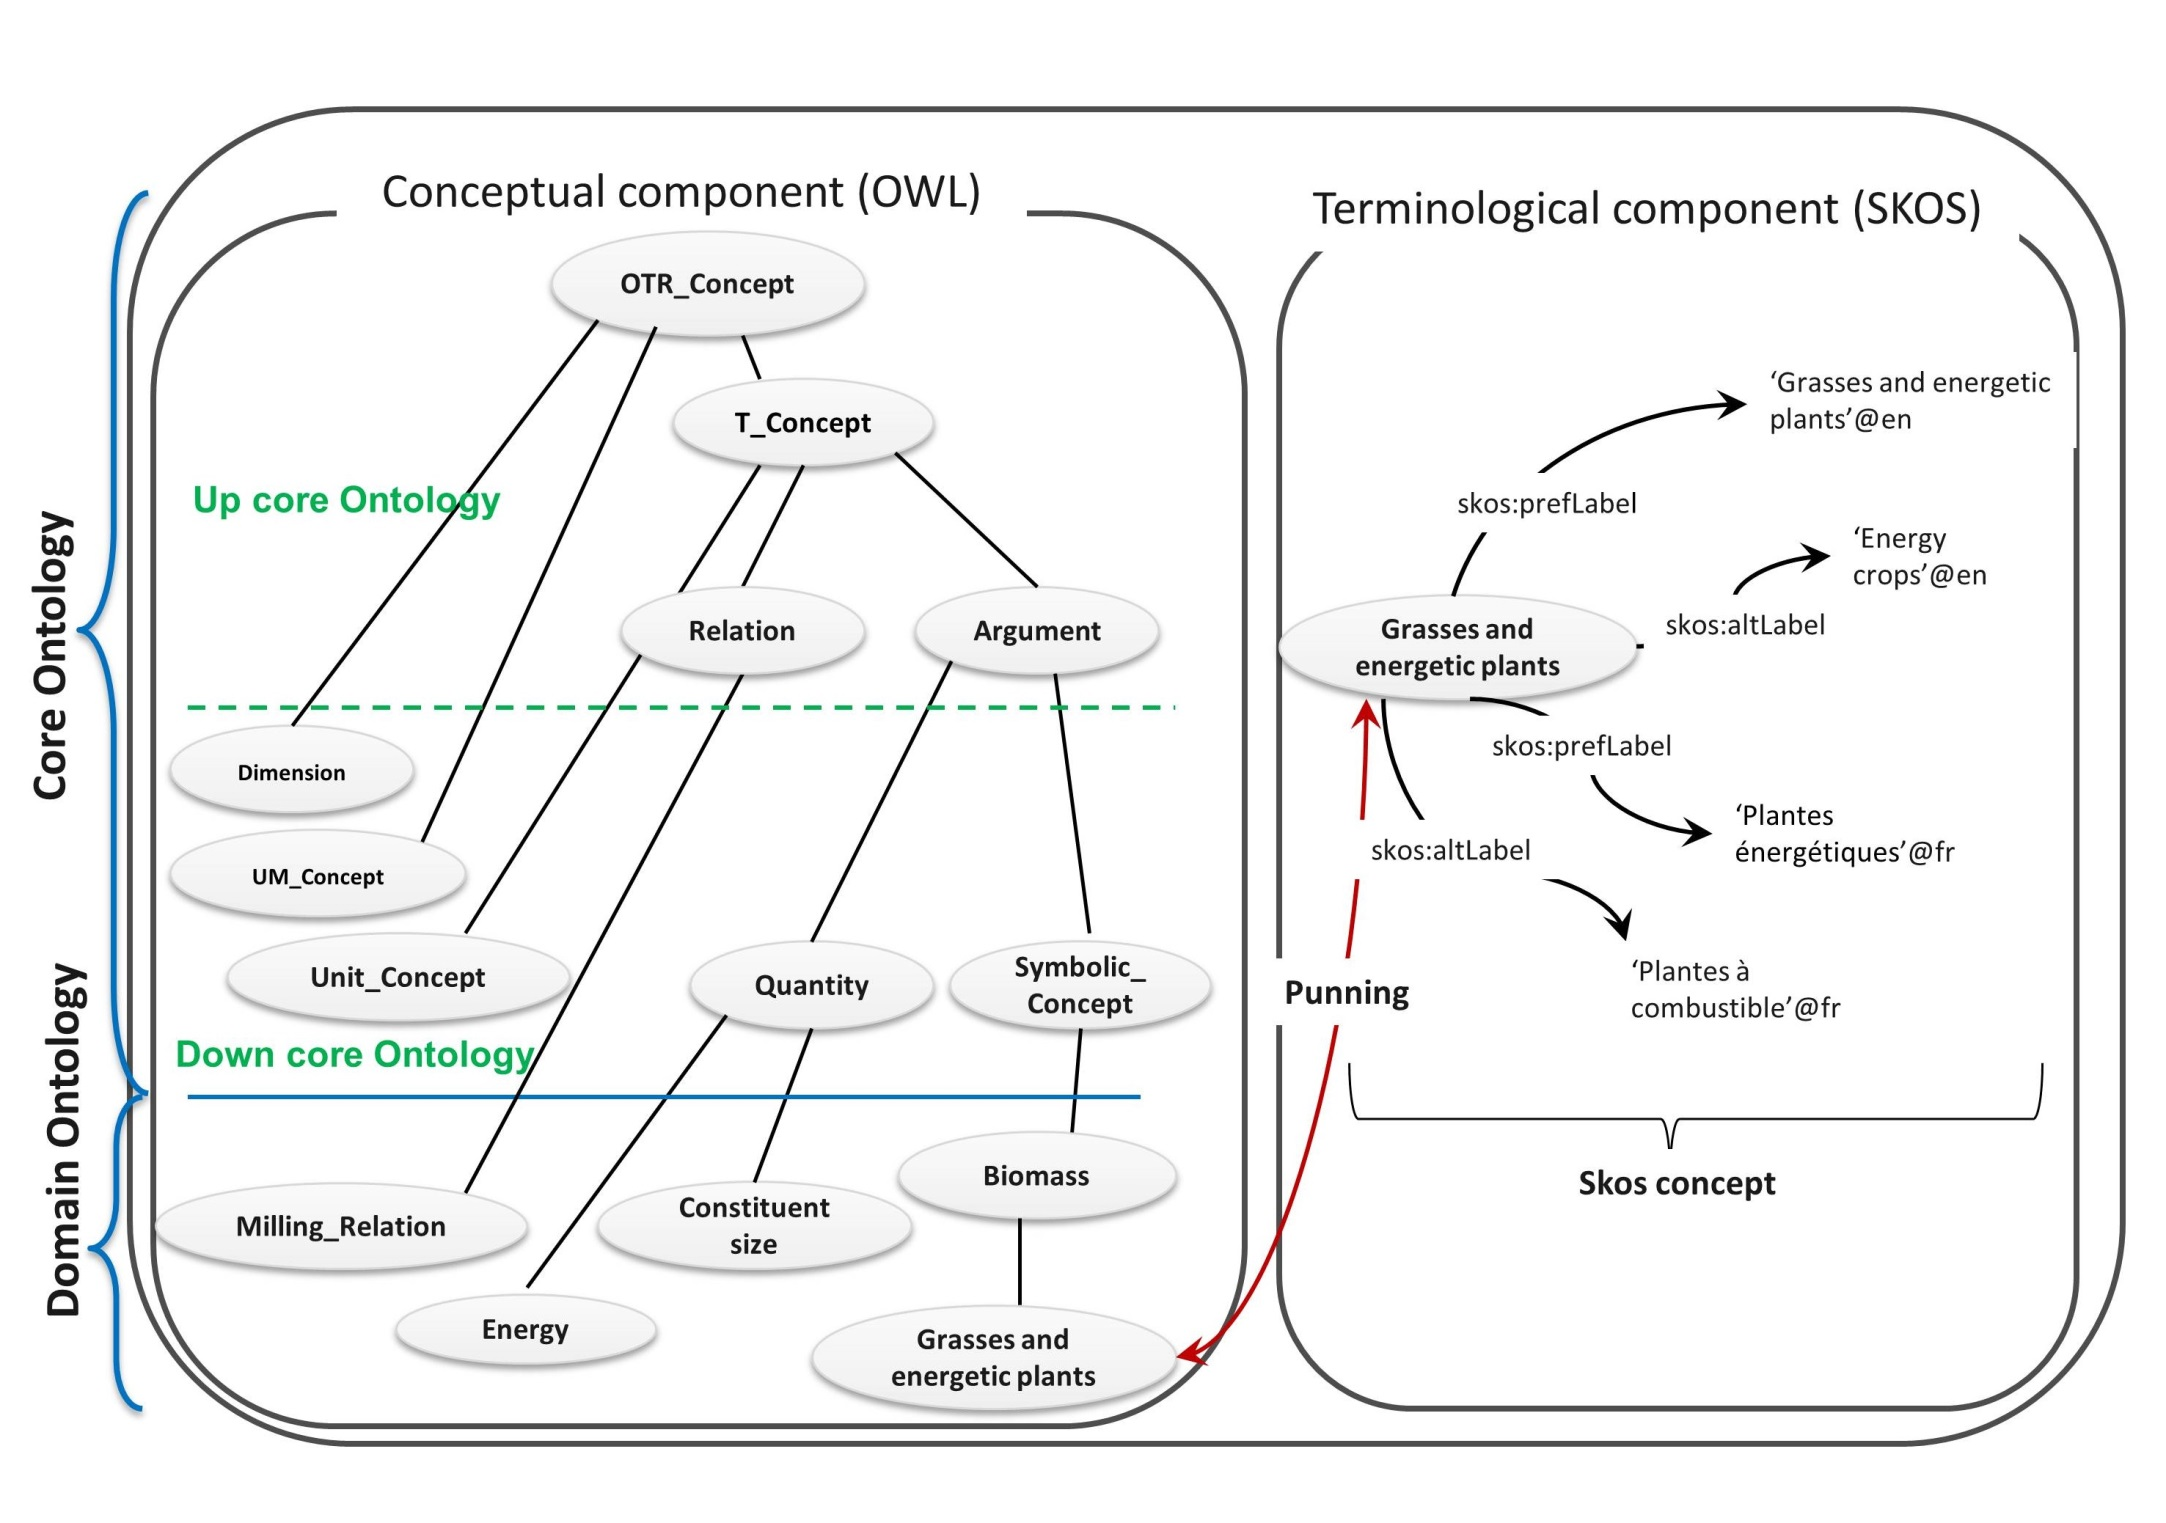
\includegraphics[width=10cm]{ontology.jpg}
  \end{center}
\end{frame}

\begin{frame}
  \frametitle{Annotated tables}
  \framesubtitle{Screenshot}

  \begin{center}
    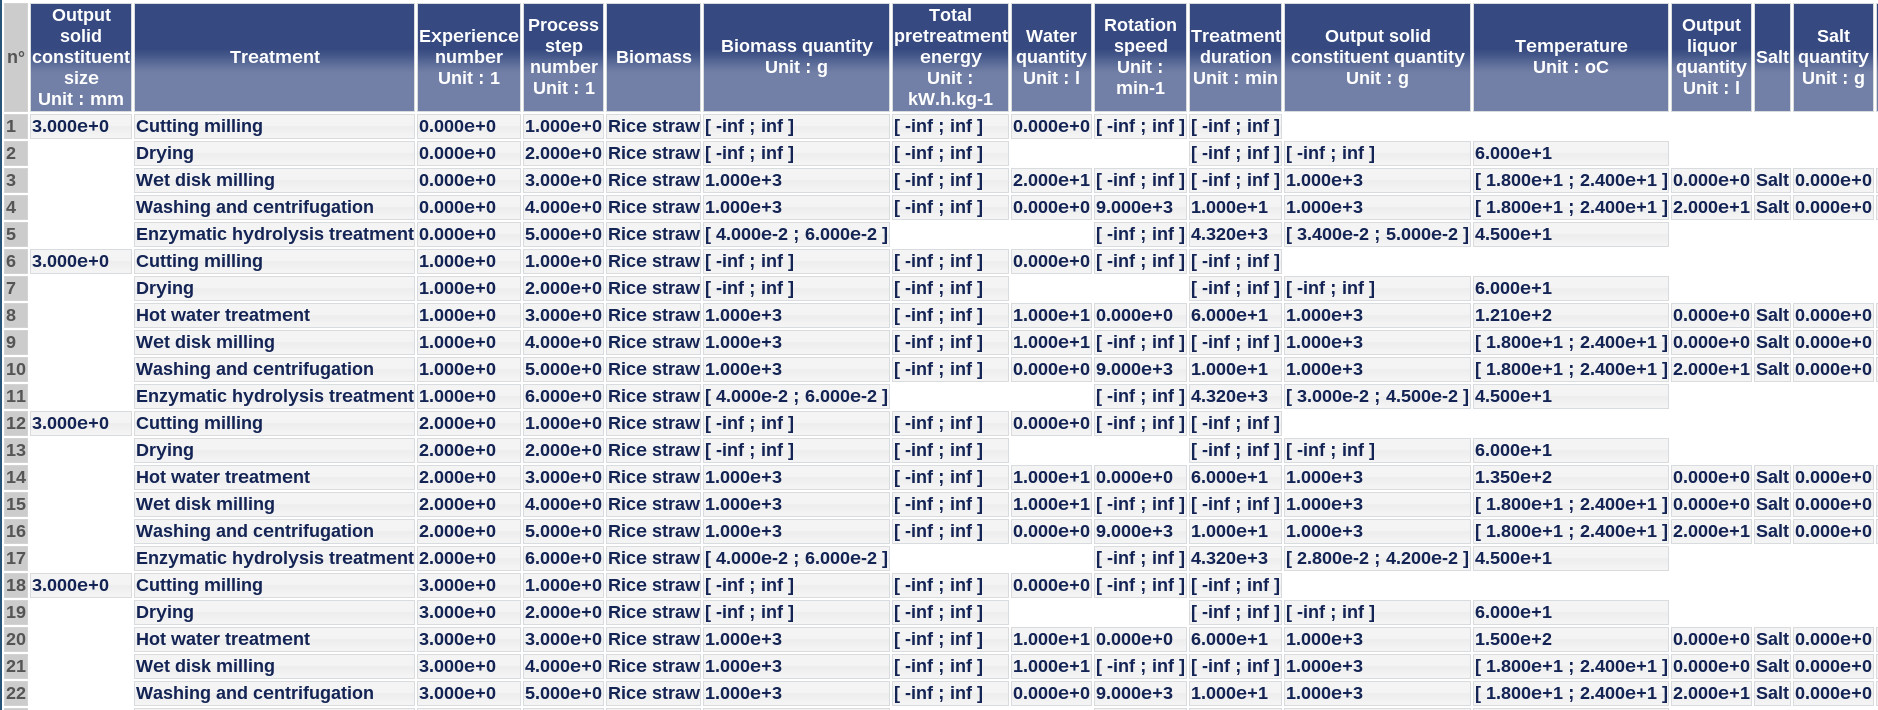
\includegraphics[width=11cm]{atweb-screenshot-table.jpg}
  \end{center}
\end{frame}

\begin{frame}
  \frametitle{Guidelines}

  \framesubtitle{Screenshot}

  \begin{center}
    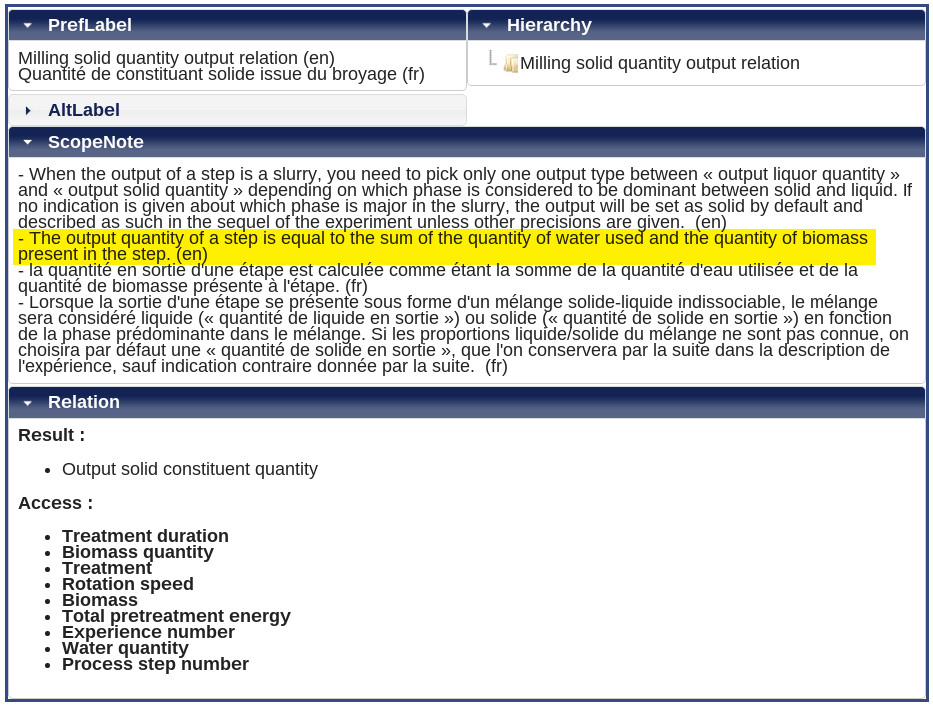
\includegraphics[width=10cm]{atweb-screenshot-guideline.jpg}
  \end{center}
\end{frame}

\begin{frame}
  \frametitle{Example guideline}
  \framesubtitle{Guideline}

  \textit{``The output quantity of a step is equal to the sum of the quantity
  of water used and the quantity of biomass present in the step.''}

  \pause

  $$output = waterInput + biomassInput$$
\end{frame}

\begin{frame}
  \frametitle{Example guideline}
  \framesubtitle{An annotated row that doesn't fulfill the guideline}

  \begin{center}
    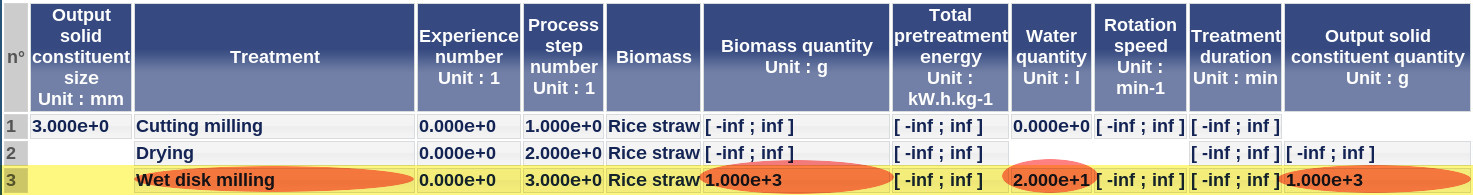
\includegraphics[width=11cm]{atweb-screenshot-row-with-relation.jpg}
  \end{center}

  \pause

  $$output = waterInput + biomassInput$$

  \pause

  {
    \color{red}
    $$1000 = 20 + 1000$$
  }
\end{frame}

\begin{frame}
  \frametitle{Example guideline}
  \framesubtitle{Underlying RDF graph}

  \begin{center}
    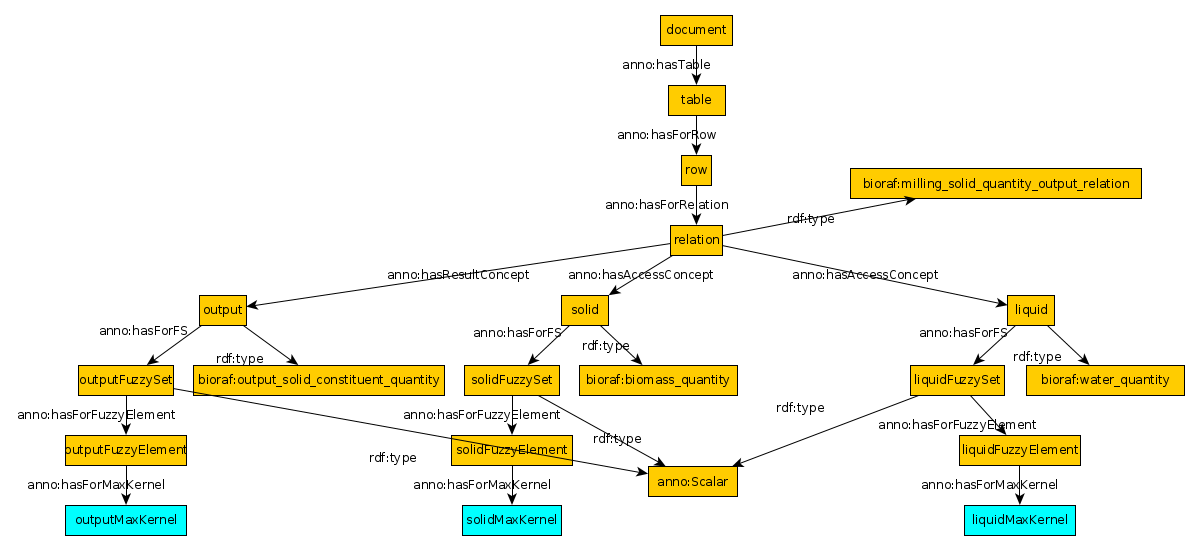
\includegraphics[width=11cm]{underlying-graph.png}
  \end{center}
\end{frame}

%%%%%%%%%%%%%%%%%%%%%%%%%%%%%%%%%%%%%%%%%%%%%%%%%%%%%%%%%%%%%%%%%%%%%%%%%%%%%%%%
% Part II: RDF data validation: survey of the state of the art                 %
%%%%%%%%%%%%%%%%%%%%%%%%%%%%%%%%%%%%%%%%%%%%%%%%%%%%%%%%%%%%%%%%%%%%%%%%%%%%%%%%

\begin{frame}
  \partslide{Part II}{RDF data validation: survey of the state of the art}
\end{frame}

\begin{frame}
  \frametitle{Shape Expressions}
  \framesubtitle{Introduction}

  \begin{itemize}
    \item It's a validation language for RDF graphs, inspired in regular
      expressions.

    \item Allows specifying patterns, or \textit{shapes}, that triples in an
      RDF graph must conform to.

    \item Lets one decide whether a RDF graph satisfies all the required shapes.

    \item Also possible to deduce which triples conform to which shapes (useful
      for classification.)

    \item Roughly comparable to what the Data Definition Language (DDL) does
      for SQL databases, or what XML Schema does for XML documents.
  \end{itemize}
\end{frame}

\begin{frame}[fragile]
  \frametitle{Shape Expressions}
  \framesubtitle{Example shape}

  \begin{Verbatim}
<UserShape> {
  ( foaf:name xsd:string |
    foaf:givenName xsd:string+ ,
    foaf:familyName xsd:string
  ),

  foaf:mbox shex:IRI ?
}
  \end{Verbatim}

  \pause

  \begin{columns}
    \column{0.5\textwidth}

    \textbf{Valid}

    \begin{Verbatim}[fontsize=\scriptsize]
:Bob
  foaf:givenName "Bob" ;
  foaf:familyName "Smith" ;
  foaf:mbox <mail:bob@example.org> .

:Thompson
  foaf:givenName "Joe", "Joseph" ;
  foaf:familyName "Thompson" ;
  foaf:mbox <mail:joe@example.org> .
    \end{Verbatim}
    \column{0.5\textwidth}

    \textbf{Invalid}

    \begin{Verbatim}[fontsize=\scriptsize, formatcom=\color{red}]
# missing :familyName.
:Anna
  foaf:givenName "Bob" ;
  foaf:mbox <mail:bob@example.org> .

# multiple foaf:names.
:Pete
  foaf:name "Peter", "Pete" ;
    \end{Verbatim}
  \end{columns}
\end{frame}

\begin{frame}[fragile]
  \frametitle{Shape Expressions}
  \framesubtitle{Semantic actions}

  \textit{Semantic actions} are arbitrary snippets of code that are executed
  after a rule is evaluated.

  \begin{itemize}
    \item Possible to express more complex validation rules (e.g. arithmetic
      constraints).

    \item Multiple programming languages can be supported, depending on the
      implementation of shape expressions.

    \item Other uses: transforming RDF triplets into different formats,
      generating forms for user interfaces automatically, etc.
  \end{itemize}

  \pause

  Example:

  \begin{Verbatim}[fontsize=\scriptsize]
    :reportedOn xsd:dateTime
        %js{ report = _.o; return true; %},
    (:reproducedBy @<EmployeeShape>,
     :reproducedOn xsd:dateTime
        %js{ return _.o.lex > report.lex; %}
        %sparql{ ?s :reportedOn ?rpt . FILTER (?o > ?rpt) %}
    )
  \end{Verbatim}
\end{frame}

\begin{frame}
  \frametitle{Shape Expressions}
  \framesubtitle{Available implementations}

  \begin{itemize}
    \item \ifnhref{ShExcala}{http://labra.github.io/ShExcala/}

    \begin{itemize}
      \item Implemented in the Scala programming language

      \item Can be used from any JVM language (good for \atweb)

      \item \textbf{Doesn't implement semantic actions}
    \end{itemize}

    \item \ifnhref{FancyShExDemo}{https://www.w3.org/2013/ShEx/FancyShExDemo}

    \begin{itemize}
      \item Implemented in the JavaScript programming language

      \item Prototype/proof-of-concept implementation of shape expressions

      \item Handles semantic actions

      \item Able to generate SPARQL queries
    \end{itemize}
  \end{itemize}
\end{frame}

\begin{frame}
  \frametitle{Shape Expressions}
  \framesubtitle{Problems}

  \begin{itemize}
    \item Semantic actions are absolutely needed if, in addition to the shape
      of our RDF graph, we want to validate the data itself (e.g. $output =
      waterInput + biomassInput$).

    \item The only available implementation for Shape Expressions that actually
      supports semantic actions is a proof of concept library built in
      JavaScript (FancyShExDemo).

    \item Hard to integrate into a JVM-based app.

    \item The Shape Expressions draft doesn't specify how semantic actions
      should be implemented, thus if we move to another Shape Expressions
      engine in the future, our semantic actions could break.
  \end{itemize}
\end{frame}

\begin{frame}
  \frametitle{SHACL}
  \framesubtitle{Introduction}

  \begin{itemize}
    \item \fnhref{SHACL}{https://www.w3.org/TR/shacl/} is a language for
      describing constraints in RDF graphs.

    \item Constraints are grouped into \textit{shapes} that apply to nodes in a
      \textit{data graph}.

    \item Shapes are described in RDF and stored in a \textit{shapes graph}.

    \item The simplest interface to a SHACL processor has two inputs:

    \begin{itemize}
      \item A data graph containing the data to be validated

      \item A shapes graph containing shape definitions
    \end{itemize}
  \end{itemize}
\end{frame}

\begin{frame}[fragile]
  \frametitle{SHACL}
  \framesubtitle{An example shape}

  \begin{columns}[t]
    \column{0.45\textwidth}

    \textbf{Shape}

    \begin{Verbatim}[fontsize=\footnotesize]
ex:UserShape
  a sh:Shape ;
  sh:property [
    sh:predicate foaf:name ;
    sh:datatype xsd:string ;
    sh:minCount 1 ;
    sh:maxCount 1 ;
  ] ;
  sh:property [
    sh:predicate foaf:mbox ;
    sh:nodeKind sh:IRI ;
    sh:minCount 1 ;
  ] .
    \end{Verbatim}

    \pause

    \column{0.55\textwidth}

    \textbf{Valid data}

    \begin{Verbatim}[fontsize=\tiny]
:User1
  a foaf:Person ;
  foaf:name "Michel Thomas" ;
  foaf:mbox <mailto:mt@example.org> .

:User2
  a foaf:Person ;
  foaf:name "Bob Lee",
  foaf:mbox <mailto:bl@example.org> ;
  foaf:mbox <mailto:bob.lee@example.org> .
    \end{Verbatim}

    \textbf{Invalid data}

    \begin{Verbatim}[fontsize=\tiny, formatcom=\color{red}]
# More than one foaf:name
:User3
  a foaf:Person ;
  foaf:name "Paul McCartney" ;
  foaf:name "Sir James Paul McCartney" ;
  foaf:mbox <mailto:paul.mccartney@example.org> .

# Missing foaf:mbox
:User4
  a foaf:Person ;
  foaf:name "Donald Knuth".
    \end{Verbatim}
  \end{columns}
\end{frame}

\begin{frame}[fragile]
  \frametitle{SHACL}
  \framesubtitle{Native constraints}

  \begin{Verbatim}[fontsize=\scriptsize]
ex:LanguageExampleShape
  a sh:Shape ;
  sh:scopeClass ex:Country ;
  sh:constraint [
    sh:message "Values must be literals with German language tag." ;
    sh:sparql """
      SELECT $this ($this AS ?subject)
                   (ex:germanLabel AS ?predicate)
                   (?value AS ?object)
      WHERE {
        $this ex:germanLabel ?value .
        FILTER (!isLiteral(?value) || !langMatches(lang(?value), "de"))
      }
      """ ;
  ] .
  \end{Verbatim}

  \pause

  \begin{columns}[t]
    \column{0.5\textwidth}

    \textbf{Valid graph}

    \begin{Verbatim}[fontsize=\footnotesize]
ex:ValidCountry
  a ex:Country ;
  ex:germanLabel "Spanien"@de .
    \end{Verbatim}

    \column{0.5\textwidth}

    \textbf{Invalid graph}

    \begin{Verbatim}[fontsize=\footnotesize, formatcom=\color{red}]
ex:InvalidCountry
  a ex:Country ;
  ex:germanLabel "Spain"@en .
    \end{Verbatim}
  \end{columns}
\end{frame}

\begin{frame}
  \frametitle{SHACL}
  \framesubtitle{A sample integrity constraint implemented in SHACL (I)}

  \vspace{0.5cm}

  \textit{``The output quantity of a step is equal to the sum of the quantity
  of water used and the quantity of biomass present in the step.''}

  $$output = waterInput + biomassInput$$

  \begin{center}
    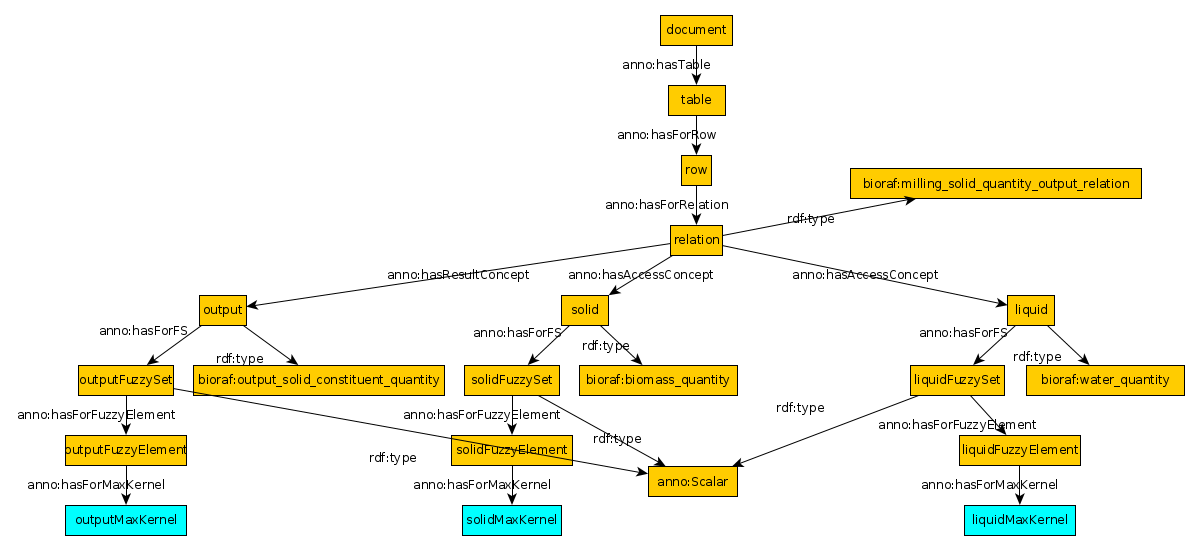
\includegraphics[width=11cm]{underlying-graph.png}
  \end{center}
\end{frame}

\begin{frame}[fragile]
  \frametitle{SHACL}
  \framesubtitle{A sample integrity constraint implemented in SHACL (II)}

  \begin{columns}[t]
    \column{0.5\textwidth}

    \begin{Verbatim}[fontsize=\tiny]
anno:MillingSolidOutputQuantityRelationshipShape
  a sh:Shape ;
  sh:scopeClass bioraf:milling_solid_quantity_output_relation ;

  sh:filterShape [
    sh:inverseProperty [
      sh:predicate anno:hasForRelation ;
      sh:valueShape [
        sh:inverseProperty [
          sh:predicate anno:hasForRow ;
          sh:valueClass anno:Table ;
          sh:minCount 1 ;
          sh:maxCount 1 ;
        ] ;
      ] ;
      sh:minCount 1 ;
      sh:maxCount 1 ;
    ]
  ] ;

  sh:property [
    sh:predicate core:hasAccessConcept ;
    sh:qualifiedValueShape [
      sh:property [
        sh:predicate rdf:type ;
        sh:hasValue bioraf:biomass_quantity
      ]
    ] ;
    sh:qualifiedMinCount 1 ;
    sh:qualifiedMaxCount 1 ;
  ] ;
    \end{Verbatim}

    \column{0.5\textwidth}

    \begin{Verbatim}[fontsize=\tiny]





sh:property [
  sh:predicate core:hasAccessConcept ;
  sh:qualifiedValueShape [
    sh:property [
      sh:predicate rdf:type ;
      sh:hasValue bioraf:water_quantity
    ]
  ] ;
  sh:qualifiedMinCount 1 ;
  sh:qualifiedMaxCount 1 ;
] ;

sh:property [
  sh:predicate core:hasResultConcept ;
  sh:valueClass bioraf:output_solid_constituent_quantity ;
  sh:minCount 1 ;
  sh:maxCount 1 ;
] ;
    \end{Verbatim}
  \end{columns}
\end{frame}

\begin{frame}[fragile]
  \frametitle{SHACL}
  \framesubtitle{A sample integrity constraint implemented in SHACL (IIII)}

  \begin{Verbatim}[fontsize=\tiny]
  sh:constraint [
    sh:predicate anno:width ;
    sh:sparql """
      SELECT $this ($this AS ?subject)
             (CONCAT("Output quantity must be the sum of the solid and liquid input quantities
                      (solid=", STR(?solid_qty),
                     ", liquid=", STR(?liquid_qty),
                     ", output=", STR(?output_qty), ")") as ?message)
      WHERE {
        $this core:hasAccessConcept ?solid ;
              core:hasAccessConcept ?liquid ;
              core:hasResultConcept ?output .

        ?solid a bioraf:biomass_quantity ;
               anno:hasForFS [a anno:Scalar ;
                              anno:hasForFuzzyElement /
                              anno:hasForMaxKernel ?solid_qty] .

        ?liquid a bioraf:water_quantity ;
                anno:hasForFS [a anno:Scalar ;
                               anno:hasForFuzzyElement /
                               anno:hasForMaxKernel ?liquid_qty] .

        ?output a bioraf:output_solid_constituent_quantity ;
                anno:hasForFS [a anno:Scalar ;
                               anno:hasForFuzzyElement /
                               anno:hasForMaxKernel ?output_qty] .

        FILTER (xsd:float(?output_qty) !=
                xsd:float(?solid_qty) + xsd:float(?liquid_qty))
      }
    """ ;
] .

  \end{Verbatim}
\end{frame}

\begin{frame}
  \frametitle{SHACL}
  \framesubtitle{Pros and cons}

  Pros:

  \begin{itemize}
    \item Constraints are represented as RDF triples; no additional storage
      medium needed.
    \item Rich core constraints vocabulary.
    \item Possible to define arbitrary constraints using SPARQL.
    \item SHACL implementation readily available (Java language).
    \item Already being used in the industry (TopQuadrant).
  \end{itemize}

  Cons:

  \begin{itemize}
    \item Constraints involving properties from different nodes require
      describing the graph structure within SPARQL queries, rendering the
      SHACL shapes redundant.
  \end{itemize}
\end{frame}

\begin{frame}
  \frametitle{Plain SPARQL}
  \framesubtitle{Idea}

  \begin{itemize}
    \item Write \fnhref{SPARQL}{https://www.w3.org/TR/sparql11-query} queries
      that implement \textit{negative constraints}: only return data that
      violates a particular constraint.

    \item In our particular case, we will return relation instances that
      violate a constraint.
  \end{itemize}
\end{frame}

\begin{frame}
  \frametitle{Plain SPARQL}
  \framesubtitle{Example constraint (I)}

  \vspace{0.5cm}

  \textit{``The output quantity of a step is equal to the sum of the quantity
  of water used and the quantity of biomass present in the step.''}

  $$output = waterInput + biomassInput$$

  \begin{center}
    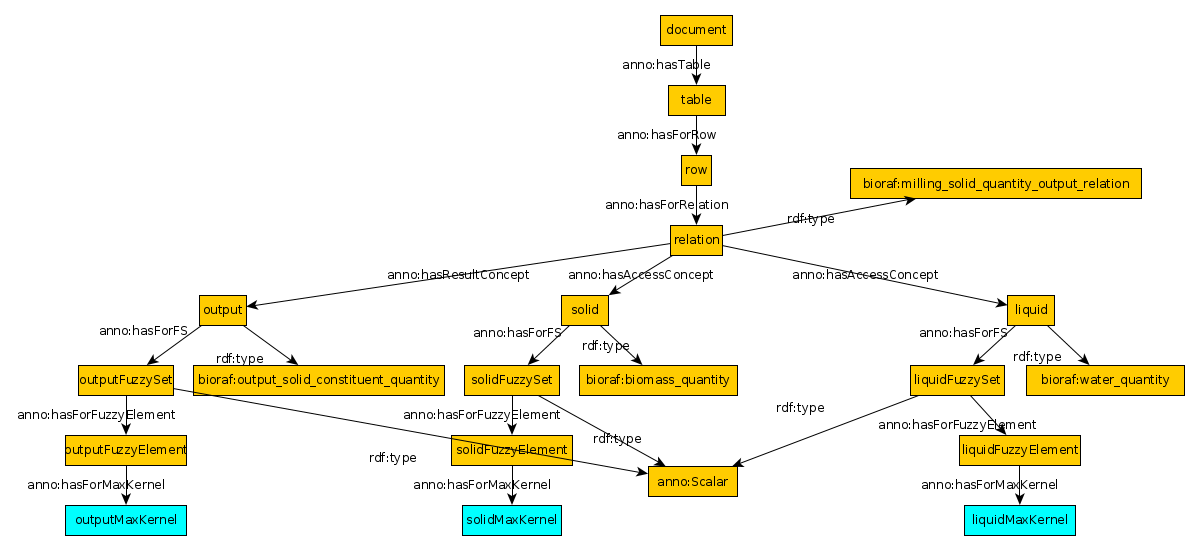
\includegraphics[width=11cm]{underlying-graph.png}
  \end{center}
\end{frame}

\begin{frame}[fragile]
  \frametitle{Plain SPARQL}
  \framesubtitle{Example constraint (II)}

  \begin{Verbatim}[fontsize=\tiny]
SELECT ?docid ?doctitle ?tableid ?tabletitle ?rownum  ?solid_qty ?liquid_qty ?output_qty WHERE {
?doc anno:hasForID ?docid ;
     dc:title ?doctitle ;
     anno:hasTable ?table .

?table anno:hasForID ?tableid ;
       dc:title ?tabletitle ;
       anno:hasForRow ?row .

?row anno:hasForRowNumber ?rownum ;
     anno:hasForRelation ?relation .

?relation a bioraf:milling_solid_quantity_output_relation ;
          core:hasAccessConcept ?solid ;
          core:hasAccessConcept ?liquid ;
          core:hasResultConcept ?output] .

?solid a bioraf:biomass_quantity ;
       anno:hasForFS [a anno:Scalar ;
                      anno:hasForFuzzyElement /
                      anno:hasForMaxKernel ?solid_qty] .

?liquid a bioraf:water_quantity ;
        anno:hasForFS [a anno:Scalar ;
                       anno:hasForFuzzyElement /
                       anno:hasForMaxKernel ?liquid_qty] .

?output a bioraf:output_solid_constituent_quantity ;
        anno:hasForFS [a anno:Scalar ;
                       anno:hasForFuzzyElement /
                       anno:hasForMaxKernel ?output_qty] .

FILTER (xsd:float(?output_qty) != xsd:float(?solid_qty) + xsd:float(?liquid_qty)) }
  \end{Verbatim}
\end{frame}

%%%%%%%%%%%%%%%%%%%%%%%%%%%%%%%%%%%%%%%%%%%%%%%%%%%%%%%%%%%%%%%%%%%%%%%%%%%%%%%%
% Part III: Implementation                                                     %
%%%%%%%%%%%%%%%%%%%%%%%%%%%%%%%%%%%%%%%%%%%%%%%%%%%%%%%%%%%%%%%%%%%%%%%%%%%%%%%%

\begin{frame}
  \partslide{Part III}{Implementation}
\end{frame}

\begin{frame}
  \begin{center}
    \Huge{Demo}
  \end{center}
\end{frame}

%%%%%%%%%%%%%%%%%%%%%%%%%%%%%%%%%%%%%%%%%%%%%%%%%%%%%%%%%%%%%%%%%%%%%%%%%%%%%%%%
% Part IV: Conclusions                                                         %
%%%%%%%%%%%%%%%%%%%%%%%%%%%%%%%%%%%%%%%%%%%%%%%%%%%%%%%%%%%%%%%%%%%%%%%%%%%%%%%%

\begin{frame}
  \partslide{Part IV}{Conclusions}
\end{frame}

\begin{frame}
  \frametitle{Conclusions}

  \begin{itemize}
    \item Shape Expressions are well suited for describing the structure of a
      graph and they can potentially be extended to do more complex kinds of
      validation via semantic actions. For the moment there are no
      feature-complete and production-ready implementations.

    \item SHACL also works well for describing the shape of a graph and is
      production-ready but the mechanism for expressing native constraints in
      SPARQL requires describing the shape of the graph again within the SPARQL
      query, rendering SHACL redundant.

    \item SPARQL remains the best suited tool for expressing the kind of
      constraints required in the \atweb platform.
  \end{itemize}
\end{frame}

\begin{frame}
  \frametitle{Future work}

  \begin{itemize}
    \item Implement \textit{positive constraints} in \atweb for classification
      purposes (i.e. return all relation instances that satisfy a set of
      conditions)

    \item Propose a specification for semantic actions in Shape Expressions

    \item Extend ShExcala (Shape Expressions engine) with a usable
      implementation of semantic actions
  \end{itemize}
\end{frame}

\begin{frame}
  \begin{center}
    \Huge{Questions?}
  \end{center}
\end{frame}

\begin{frame}
  \begin{center}
    \Huge{Thanks!}
  \end{center}
\end{frame}

% \begin{frame}
%   \frametitle{Motivation}
%   \framesubtitle{Problem statement}
%
%   \pause
%
%   \begin{itemize}
%     \item We're trying to answer questions that require consulting
%       heterogeneous data sources.
%
%     \pause
%
%     \begin{itemize}
%       \item Literature with inconsistent, semi-structured data.
%
%       \pause
%
%       \item No standard naming convention.
%
%       \pause
%
%       \item No information about the reliability of the data sources.
%
%       \pause
%
%       \item Each data source has its specific browsing/querying mechanism (no
%         common interface.)
%     \end{itemize}
%   \end{itemize}
% \end{frame}
%
% \begin{frame}
%   \frametitle{Motivation}
%   \framesubtitle{Sample problem domain: \textbf{biorefinery}}
%
%   \begin{itemize}
%     \item Ligno-cellulosic biomass pre-treatment before enzymatic hydrolysis is
%       an essential step to obtain good yields.
%
%     \pause
%
%     \item Several pre-treatment principles available, but \textbf{no clear
%       criteria on how to choose the best one} taking into account environmental
%       sustainability for a given biomass and biorefinery product (e.g.
%       glucose.)
%   \end{itemize}
% \end{frame}
%
% \begin{frame}
%   \frametitle{Proposed solution}
%
%   \begin{itemize}
%     \item Represent scientific knowledge with ontologies using recommended
%       standardized tools and languages for such purposes (semantic web
%       technologies, RDF(S), OWL, etc.)
%
%     \pause
%
%     \item Develop an ontology and data management web application (e.g. the
%       \textbf{@Web platform}) that makes it easy for scientists to introduce
%       data from scientific publications into an ontology, execute queries
%       against an ontology, etc.
%
%     \pause
%
%     \item Create integrity constraints to automatically detect inconsistencies
%       and errors in scientific publications and to automatically classify
%       publications according to their topics.
%
%     \pause
%
%     \begin{itemize}
%       \item \textit{The focus of my internship!}
%     \end{itemize}
%
%   \end{itemize}
% \end{frame}
%
% \begin{frame}
%   \frametitle{An example of a termino-ontological resource}
%   \framesubtitle{Taken from the biorefinery application}
%
%   \begin{center}
%     \includegraphics[width=10cm]{termino-ontological-resource.jpg}
%   \end{center}
% \end{frame}
%
% \begin{frame}
%   \frametitle{Design goals for the core ontology}
%
%   \begin{itemize}
%     \item \textbf{Simple} so as to make the annotator's task easier.
%
%     \pause
%
%     \item \textbf{Generic} enough so that the approach can be applied to
%       different, unrelated domains.
%
%     \pause
%
%     \begin{itemize}
%       \item Proven in the domains of biorefinery and packaging selection.
%     \end{itemize}
%   \end{itemize}
% \end{frame}
%
% \begin{frame}
%   \frametitle{A sample relation}
%   \framesubtitle{Also from the biorefinery domain}
%
%   \begin{center}
%     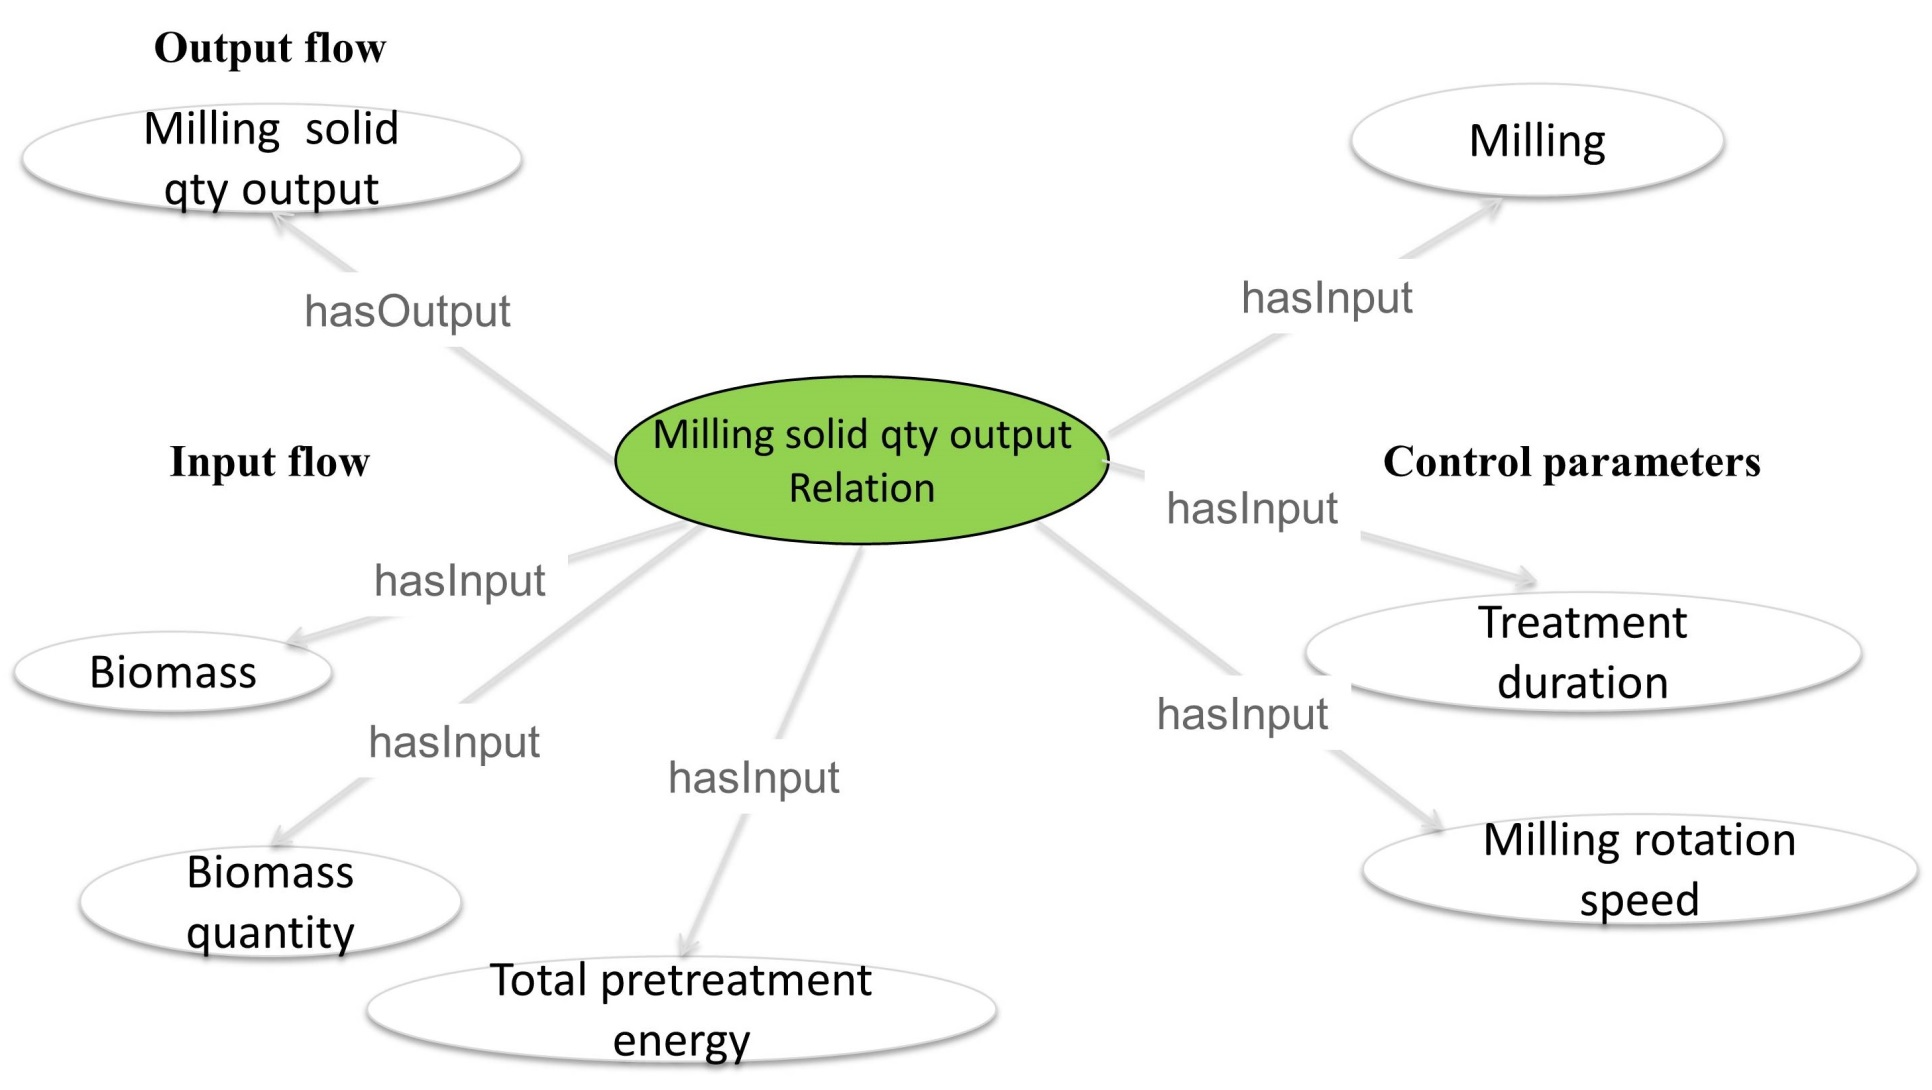
\includegraphics[width=10cm]{relation.jpg}
%   \end{center}
% \end{frame}
%
% \begin{frame}
%   \frametitle{The \textbf{@Web} platform}
%   \framesubtitle{Exploring an ontology}
%
%   \begin{center}
%     \includegraphics[width=8cm]{atweb-ontology.jpg}
%   \end{center}
% \end{frame}
%
% \begin{frame}
%   \frametitle{The \textbf{@Web} platform}
%   \framesubtitle{Browsing documents}
%
%   \begin{center}
%     \includegraphics[width=10cm]{atweb-document.jpg}
%   \end{center}
% \end{frame}
%
% \begin{frame}
%   \frametitle{The \textbf{@Web} platform}
%   \framesubtitle{Querying an ontology: defining the search scope}
%
%   \begin{center}
%     \includegraphics[width=10cm]{atweb-query-1.jpg}
%   \end{center}
% \end{frame}
%
% \begin{frame}
%   \frametitle{The \textbf{@Web} platform}
%   \framesubtitle{Querying an ontology: search parameters}
%
%   \begin{center}
%     \includegraphics[width=10cm]{atweb-query-2.jpg}
%   \end{center}
% \end{frame}
%
% \begin{frame}
%   \frametitle{The \textbf{@Web} platform}
%   \framesubtitle{Querying an ontology: executing a query}
%
%   \begin{center}
%     \includegraphics[width=10cm]{atweb-query-3.jpg}
%   \end{center}
% \end{frame}
%
% \begin{frame}
%   \frametitle{The \textbf{@Web} platform}
%   \framesubtitle{Querying an ontology: results}
%
%   \begin{center}
%     \includegraphics[width=10cm]{atweb-query-4.jpg}
%   \end{center}
% \end{frame}
%
% \begin{frame}
%   \frametitle{The annotator's task}
%
%   \begin{itemize}
%     \item Given a scientific publication and a desired ontology, capture data
%       from the publication using the appropriate concepts in the ontology.
%
%     \pause
%
%     \item Create and update concepts in the ontology as they're discovered
%       during the annotation process (i.e. in an iterative fashion.)
%
%     \pause
%
%     \item Write and edit \textbf{guidelines} associated to each concept
%       explaining when and how a concept should be used.
%   \end{itemize}
% \end{frame}
%
% \begin{frame}
%   \frametitle{An example of data captured from a scientific publication}
%
%   \begin{center}
%     \includegraphics[width=11cm]{table.jpg}
%   \end{center}
% \end{frame}
%
% \begin{frame}
%   \frametitle{A sample guideline}
%
%   \begin{center}
%     \includegraphics[width=10cm]{guideline.jpg}
%   \end{center}
% \end{frame}
%
% \begin{frame}
%   \frametitle{Some sample guidelines that can be easily translated into SPARQL
%   constraints}
%   \framesubtitle{Integrity constraints}
%
%   \begin{itemize}
%     \item \textit{``The output quantity of a step is equal to the sum of the
%       quantity of water used and the quantity of biomass present in the
%     step.''}
%
%     \pause
%
%     \item \textit{``The second milling step must give an “Output solid
%       constituent size” smaller than 0,5-1 mm.''}
%   \end{itemize}
% \end{frame}
%
% \begin{frame}
%   \frametitle{Some sample guidelines that can be easily translated into SPARQL
%   constraints}
%   \framesubtitle{Classification constraints}
%
%   \begin{itemize}
%     \item \textit{``Topic Bioref-PM-PC-UFM-PS : included experiments are
%       composed of a pre-milling step, followed by a physico-chemical treatment,
%     then by an ultrafine milling step (ball milling, wet disk milling, etc.), a
%   press and separation step (washing and filtration), and finally the enzymatic
% hydrolysis step. This topic requires a press and separation step because there
% are a lot of effluents in the physico-chemical step or because the milling is
% made with effluent. The second milling step must give an “Output solid
% constituent size” smaller than 0,5-1 mm. (en)''}
%   \end{itemize}
% \end{frame}
%
% \begin{frame}
%   \frametitle{Examples of guidelines that \textbf{cannot} be easily
%   translated into SPARQL constraints}
%
%   \begin{itemize}
%     \item \textit{``In all treatments, when the authors indicate ``overnight'',
%       we considered a duration treatment between 10 and 15 hours''}
%
%     \pause
%
%     \item \textit{``Furthermore, we consider that the glucose rate equals to
%       glucan rate divided by 0.9.''}
%   \end{itemize}
% \end{frame}
%
% \begin{frame}
%   \frametitle{Statistics}
%   \framesubtitle{A promising approach}
%
%   In the biorefinery ontology alone we have:
%
%   \begin{itemize}
%     \item 11 occurrences of the phrase \textit{``equal to''}
%     \item 5 occurrences of the phrase \textit{``equals to''}
%     \item 11 occurrences of the phrase \textit{``sum of''}
%     \item 3 occurrences of the phrase \textit{``divided by''}
%     \item 2 occurrences of the phrase \textit{``multiplied by''}
%   \end{itemize}
%
%   spread across guidelines associated with 30 relation concepts.
%
%   \vspace{1em}
%
%   \textbf{At least 10 of them can be easily translated into SPARQL constraints.}
% \end{frame}

\end{document}
